% you don't need a template
% use the following one

\documentclass{report}

\usepackage{graphicx}
\usepackage{float}
\usepackage{subcaption}
\graphicspath{{img/}}
\usepackage[a4paper, top=2cm, bottom=2cm, left=3cm, right=3cm]{geometry}


\usepackage{listings}
\lstset{language=Python, basicstyle=\ttfamily\small, frame=single, breaklines=true}

\title{A Labwork 6 Report}
\author{Luc Lacotte}
\date{}

\begin{document}

\maketitle

\section{Introduction}
This labwork is about mapping function using GPU.

\section{Binarization}

\begin{lstlisting}
@cuda.jit
def image_binarization(src, dst, threshold):
    tidx = cuda.threadIdx.x + cuda.blockIdx.x * cuda.blockDim.x
    tidy = cuda.threadIdx.y + cuda.blockIdx.y * cuda.blockDim.y
    if tidy >= src.shape[0] or tidx >= src.shape[1]:
        return
    if src[tidy, tidx] > threshold:
        dst[tidy, tidx] = 255
    else:
        dst[tidy, tidx] = 0
\end{lstlisting}

\begin{figure}[H]
\centering
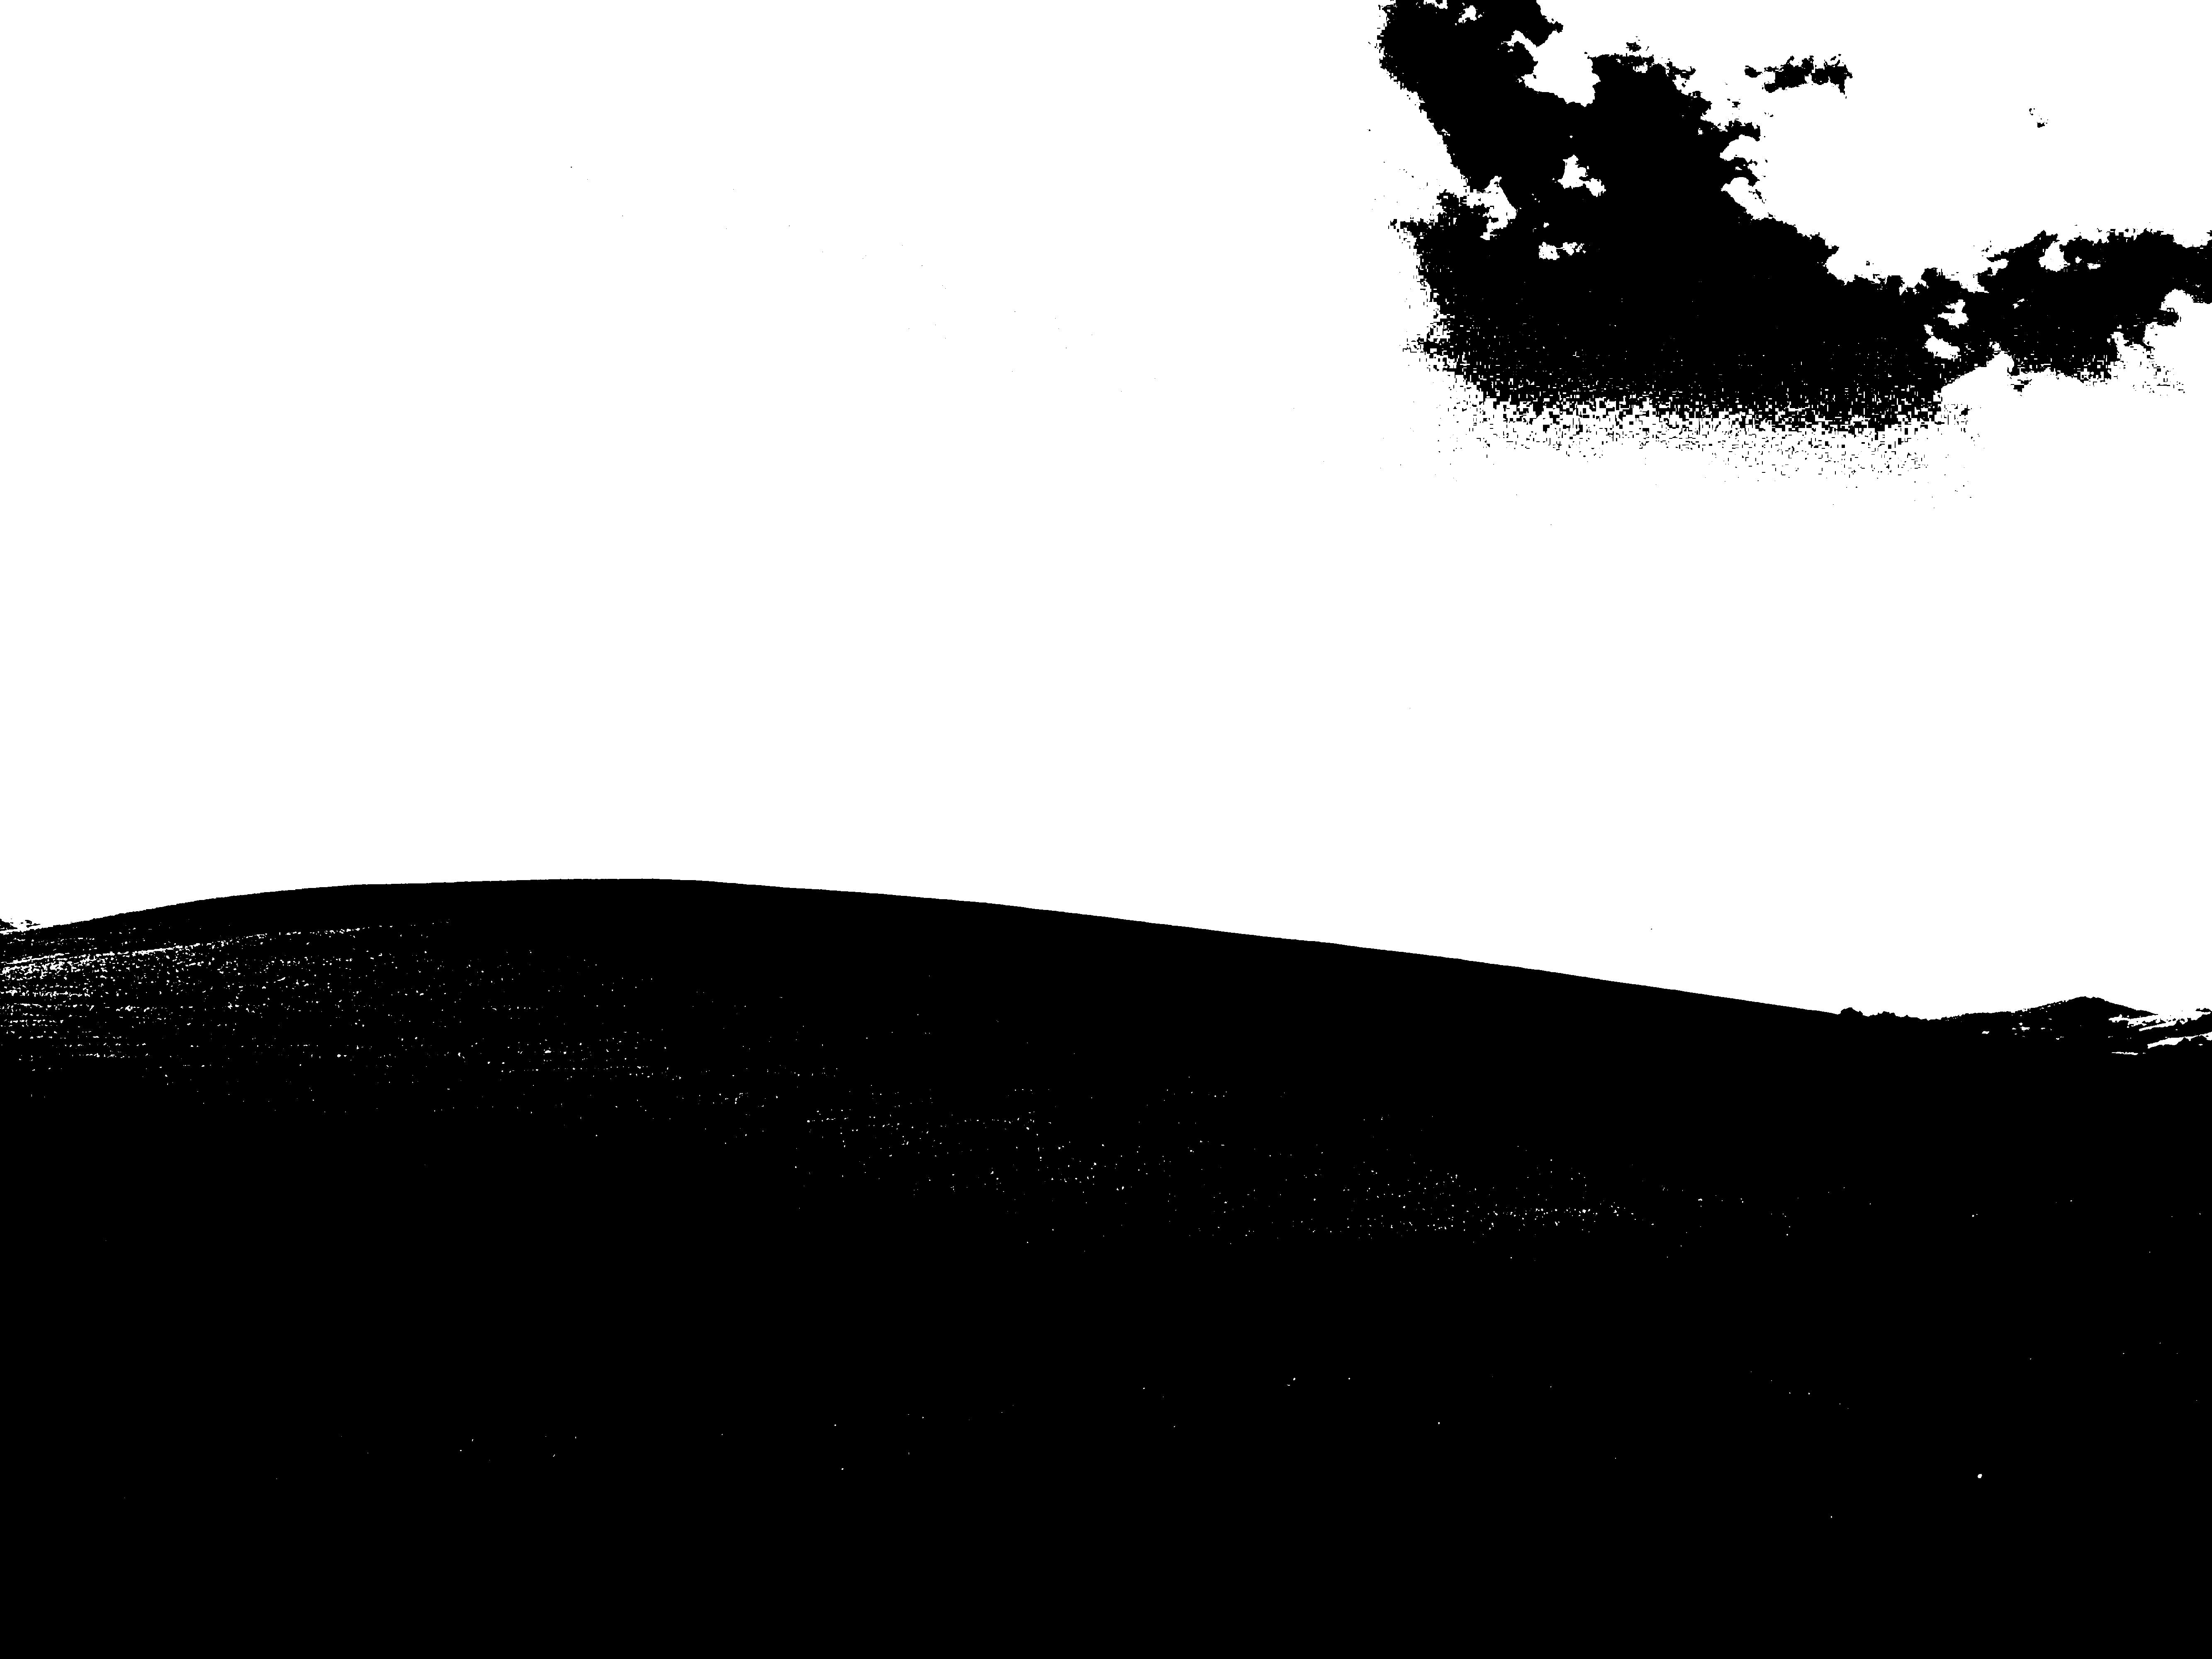
\includegraphics[width=0.7\textwidth]{binarized_img.png}
\caption{Binarized image using a threshold of 128.}
\end{figure}

\section{Brightness control}

\begin{lstlisting}
@cuda.jit
def brightness_control(src, dst, value):
    tidx = cuda.threadIdx.x + cuda.blockIdx.x * cuda.blockDim.x
    tidy = cuda.threadIdx.y + cuda.blockIdx.y * cuda.blockDim.y
    if tidy >= src.shape[0] or tidx >= src.shape[1]:
        return
    for i in range(3):
        dst[tidy, tidx, i] = min(max(src[tidy, tidx, i] + value, 0), 255)
\end{lstlisting}

min(max(...., 0), 255) is used to ensure that the pixel values remain within the valid range of 0 to 255 after adding the brightness value.

\begin{figure}[H]
\centering
\begin{subfigure}{0.48\textwidth}
\centering
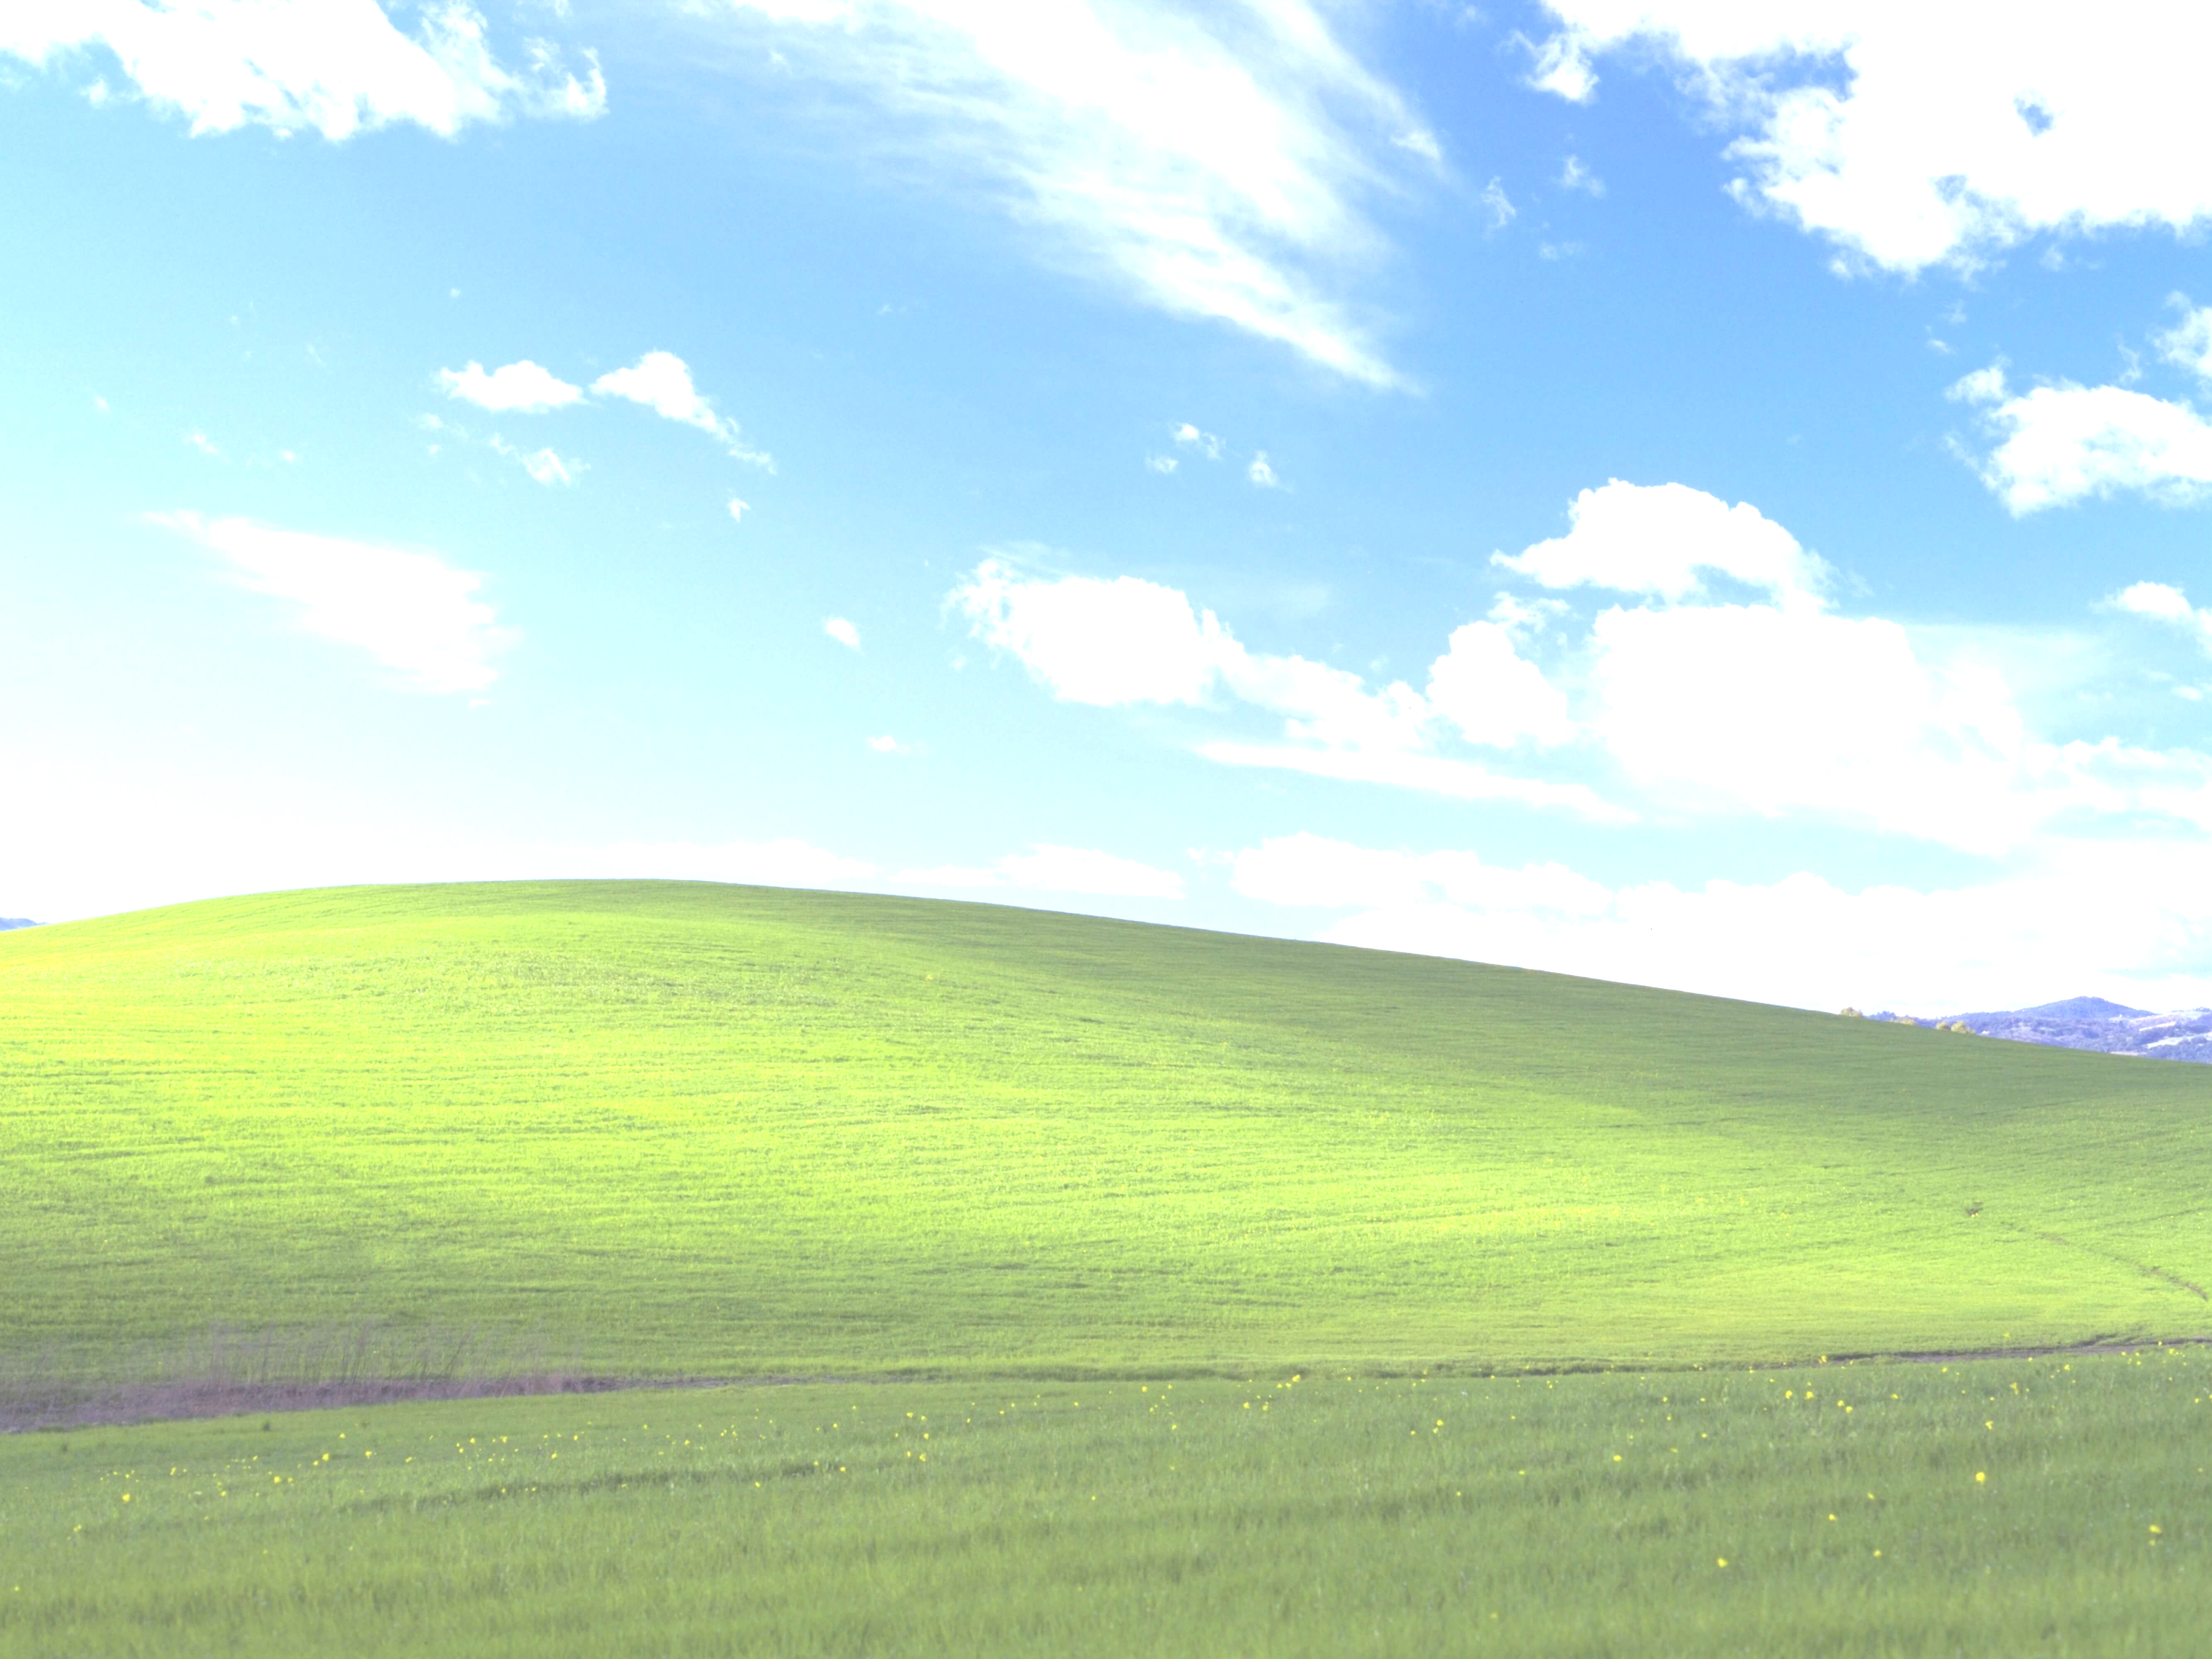
\includegraphics[width=\textwidth]{add_100.png}
\caption{Brightness $+100$.}
\end{subfigure}
\hfill
\begin{subfigure}{0.48\textwidth}
\centering
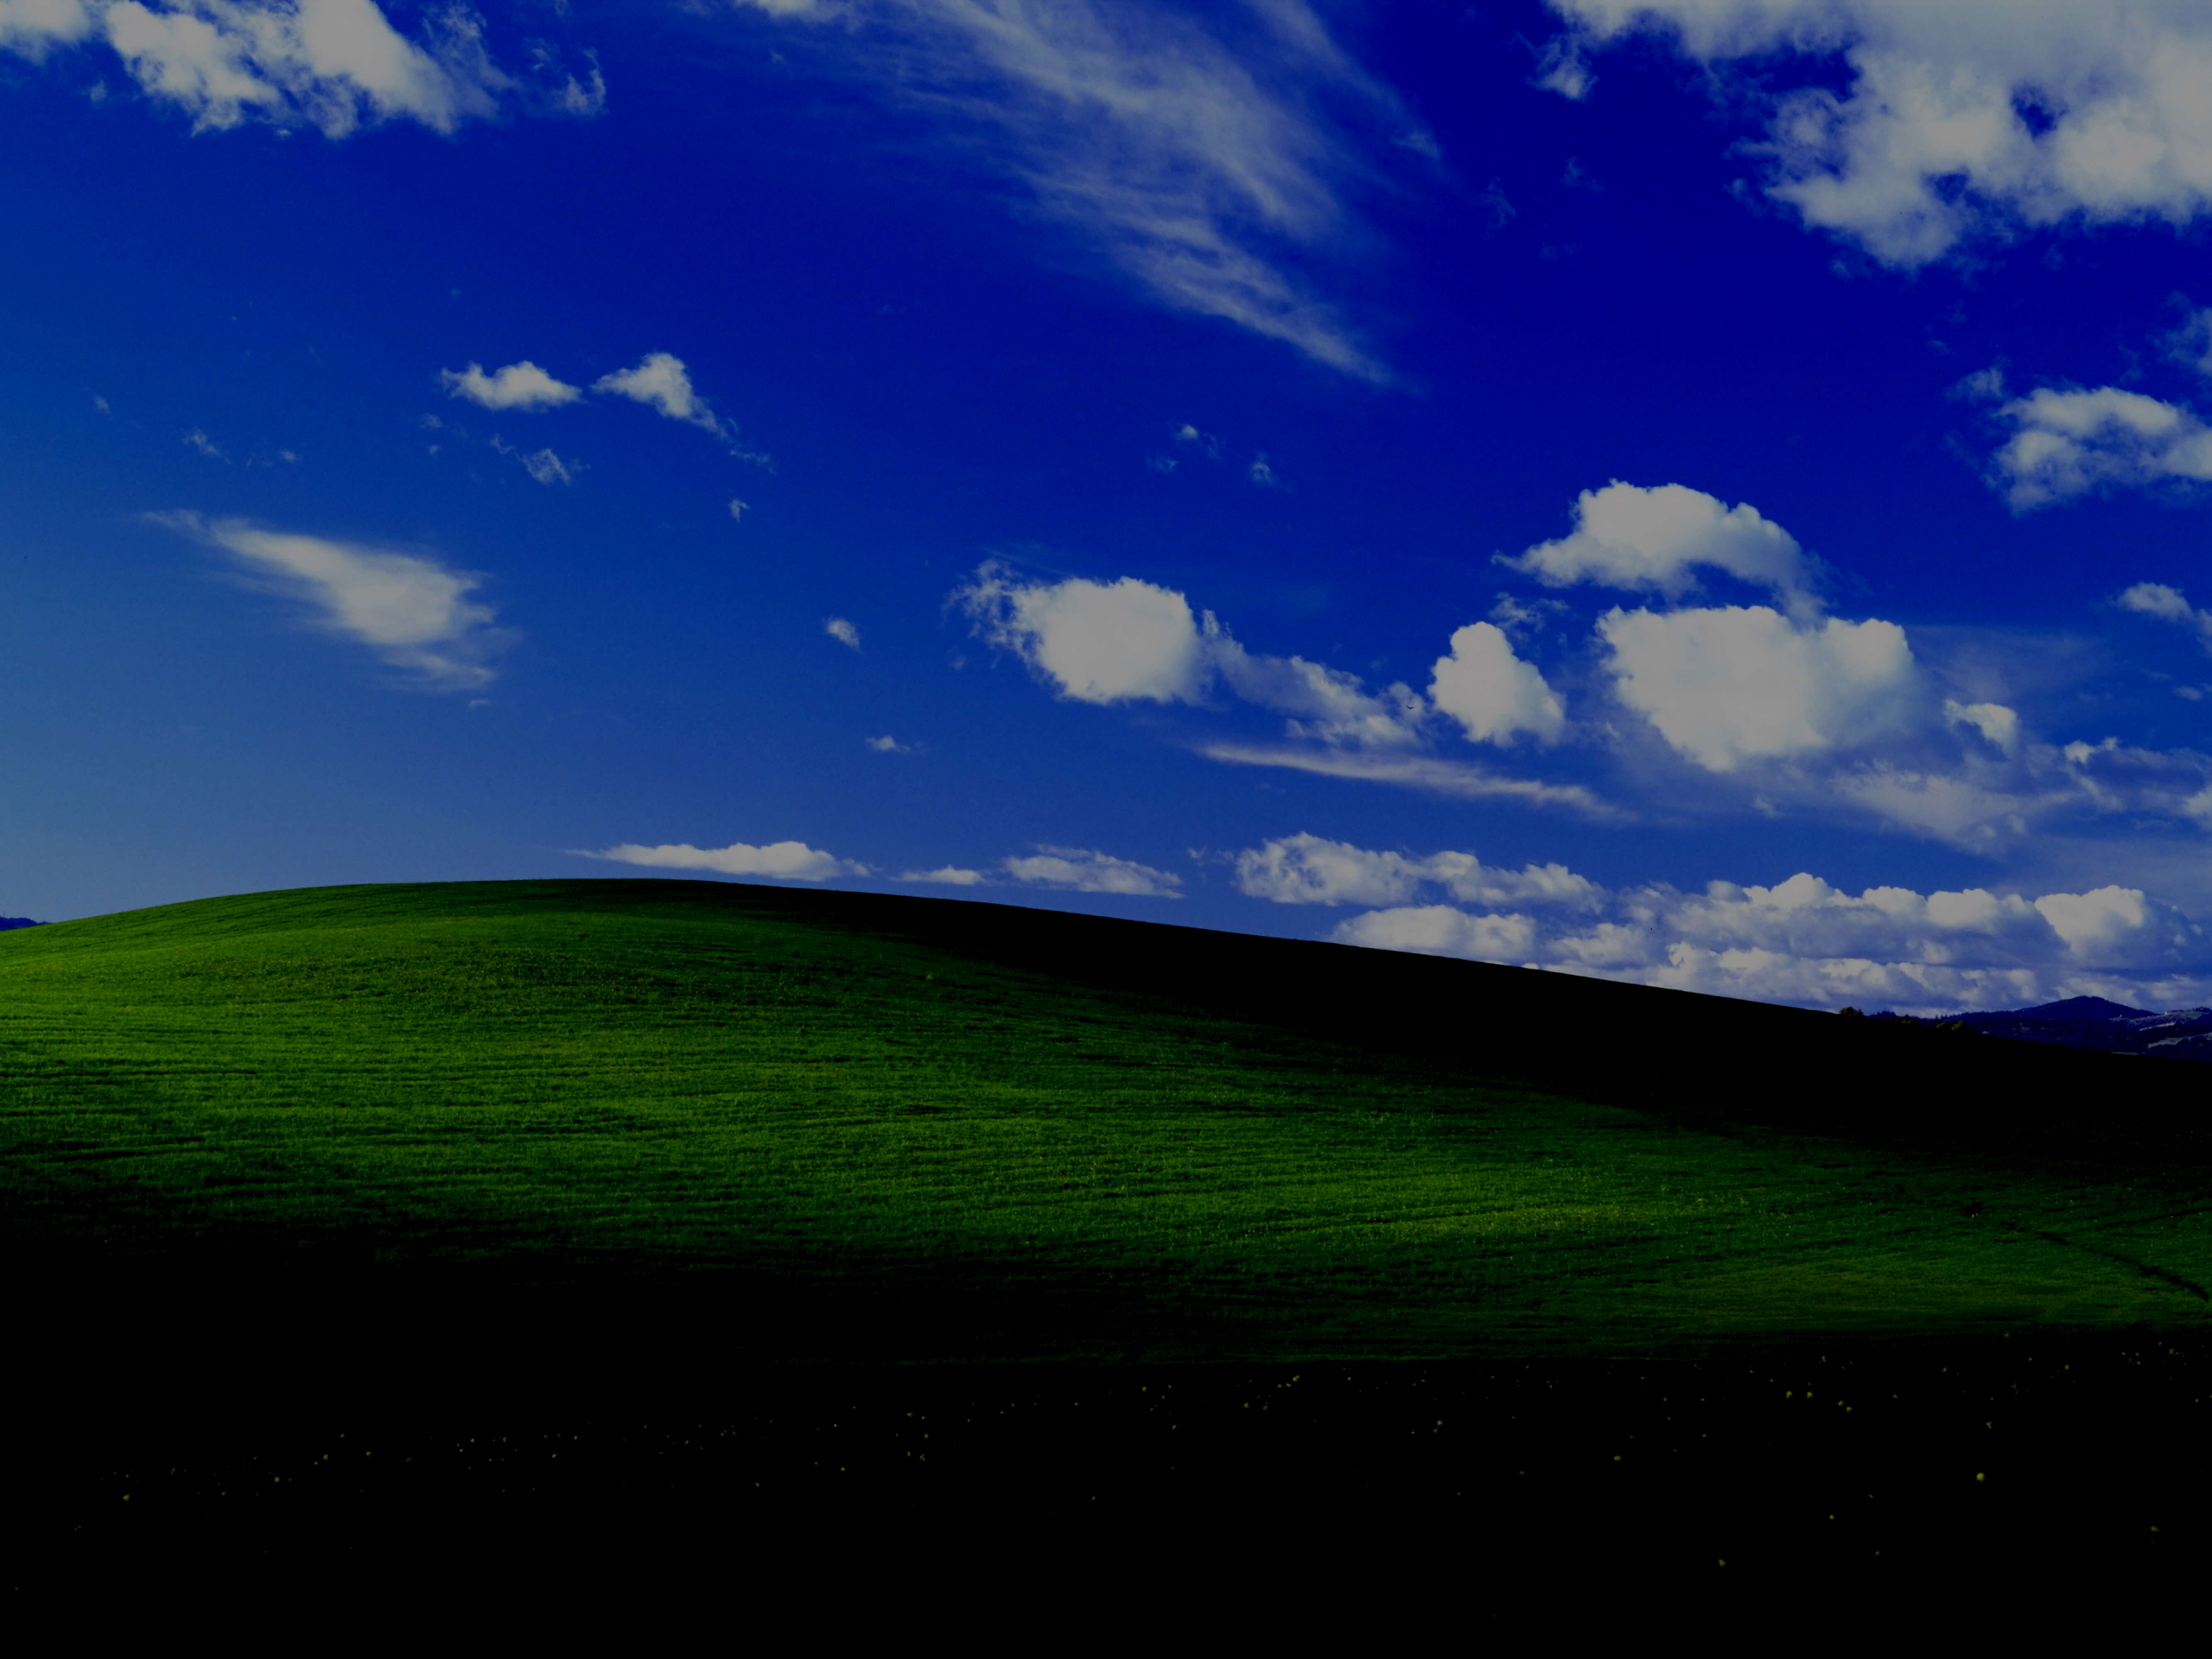
\includegraphics[width=\textwidth]{remove_100.png}
\caption{Brightness $-100$.}
\end{subfigure}
\caption{Brightness control.}
\end{figure}

\section{Blending}
\begin{lstlisting}
@cuda.jit
def blend_two_images(src1, src2, dst, c):
    tidx = cuda.threadIdx.x + cuda.blockIdx.x * cuda.blockDim.x
    tidy = cuda.threadIdx.y + cuda.blockIdx.y * cuda.blockDim.y
    if tidy >= src1.shape[0] or tidx >= src1.shape[1]:
        return
    for i in range(3):
        dst[tidy, tidx, i] = int(src1[tidy, tidx, i] * c + src2[tidy, tidx, i] * (1 - c))
\end{lstlisting}

\begin{figure}[H]
\centering
\begin{subfigure}{0.32\textwidth}
\centering
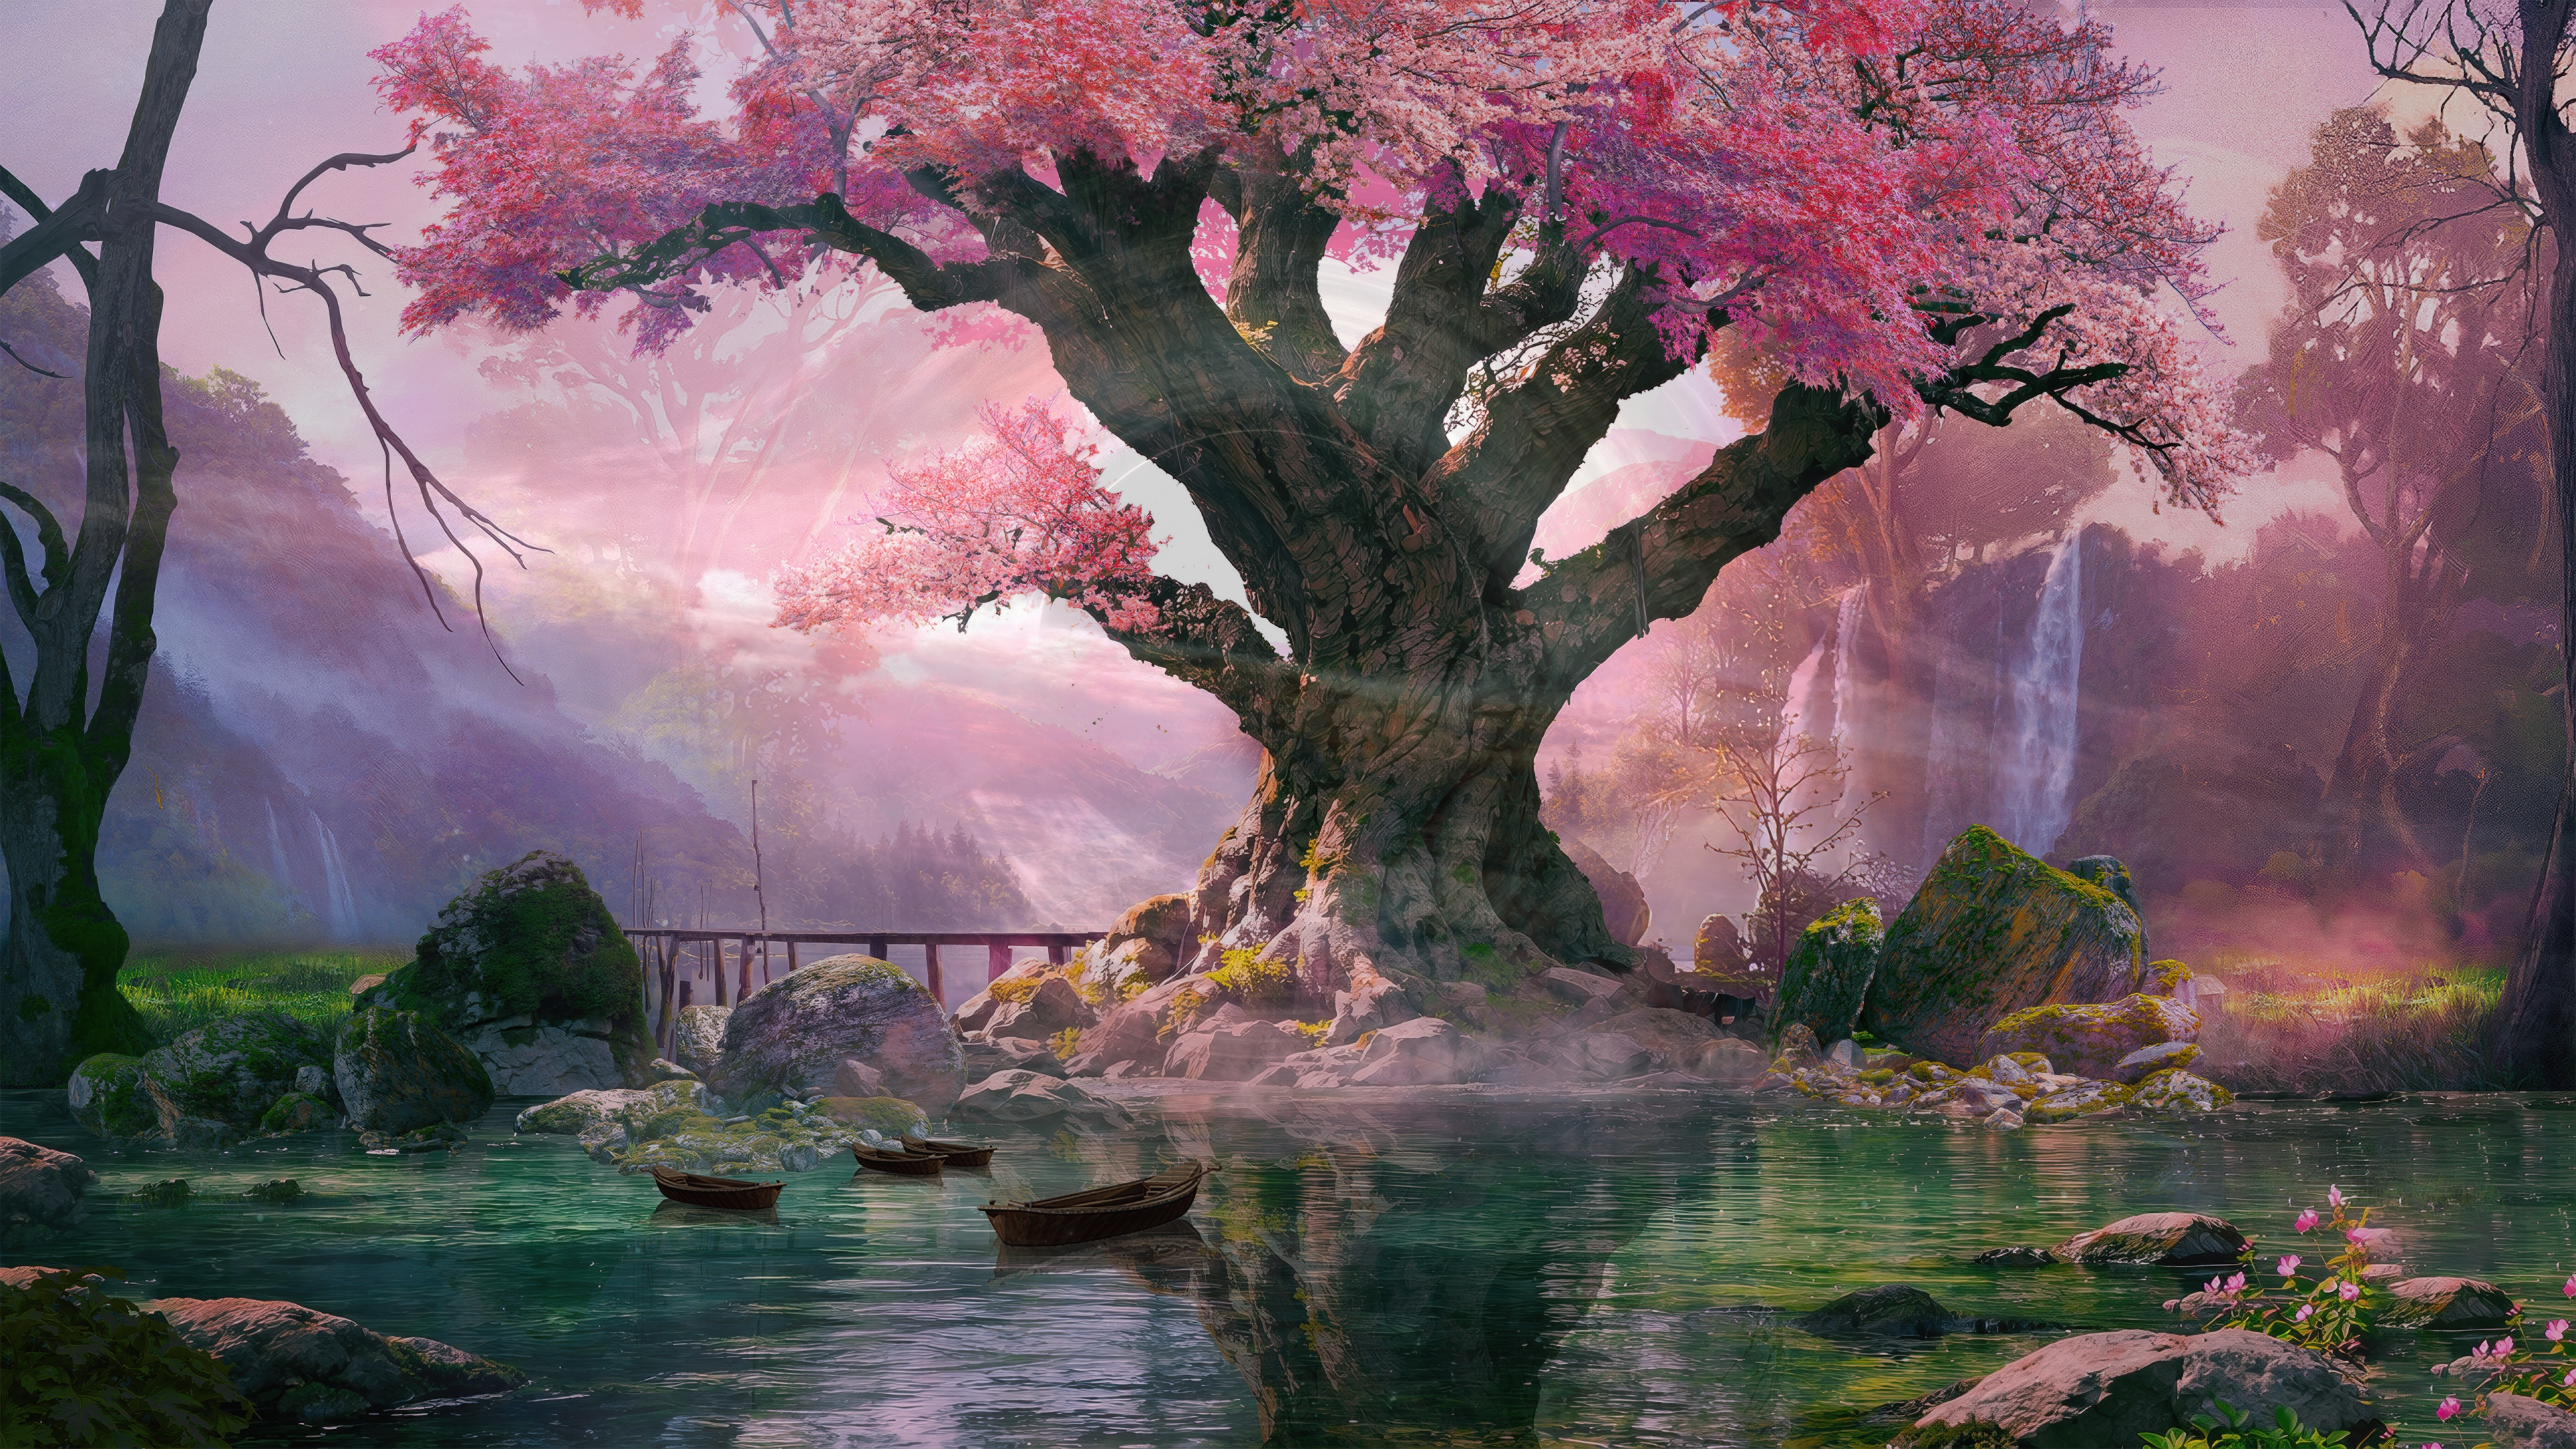
\includegraphics[width=\textwidth]{blend_0.2.png}
\caption{$c = 0.2$}
\end{subfigure}
\hfill
\begin{subfigure}{0.32\textwidth}
\centering
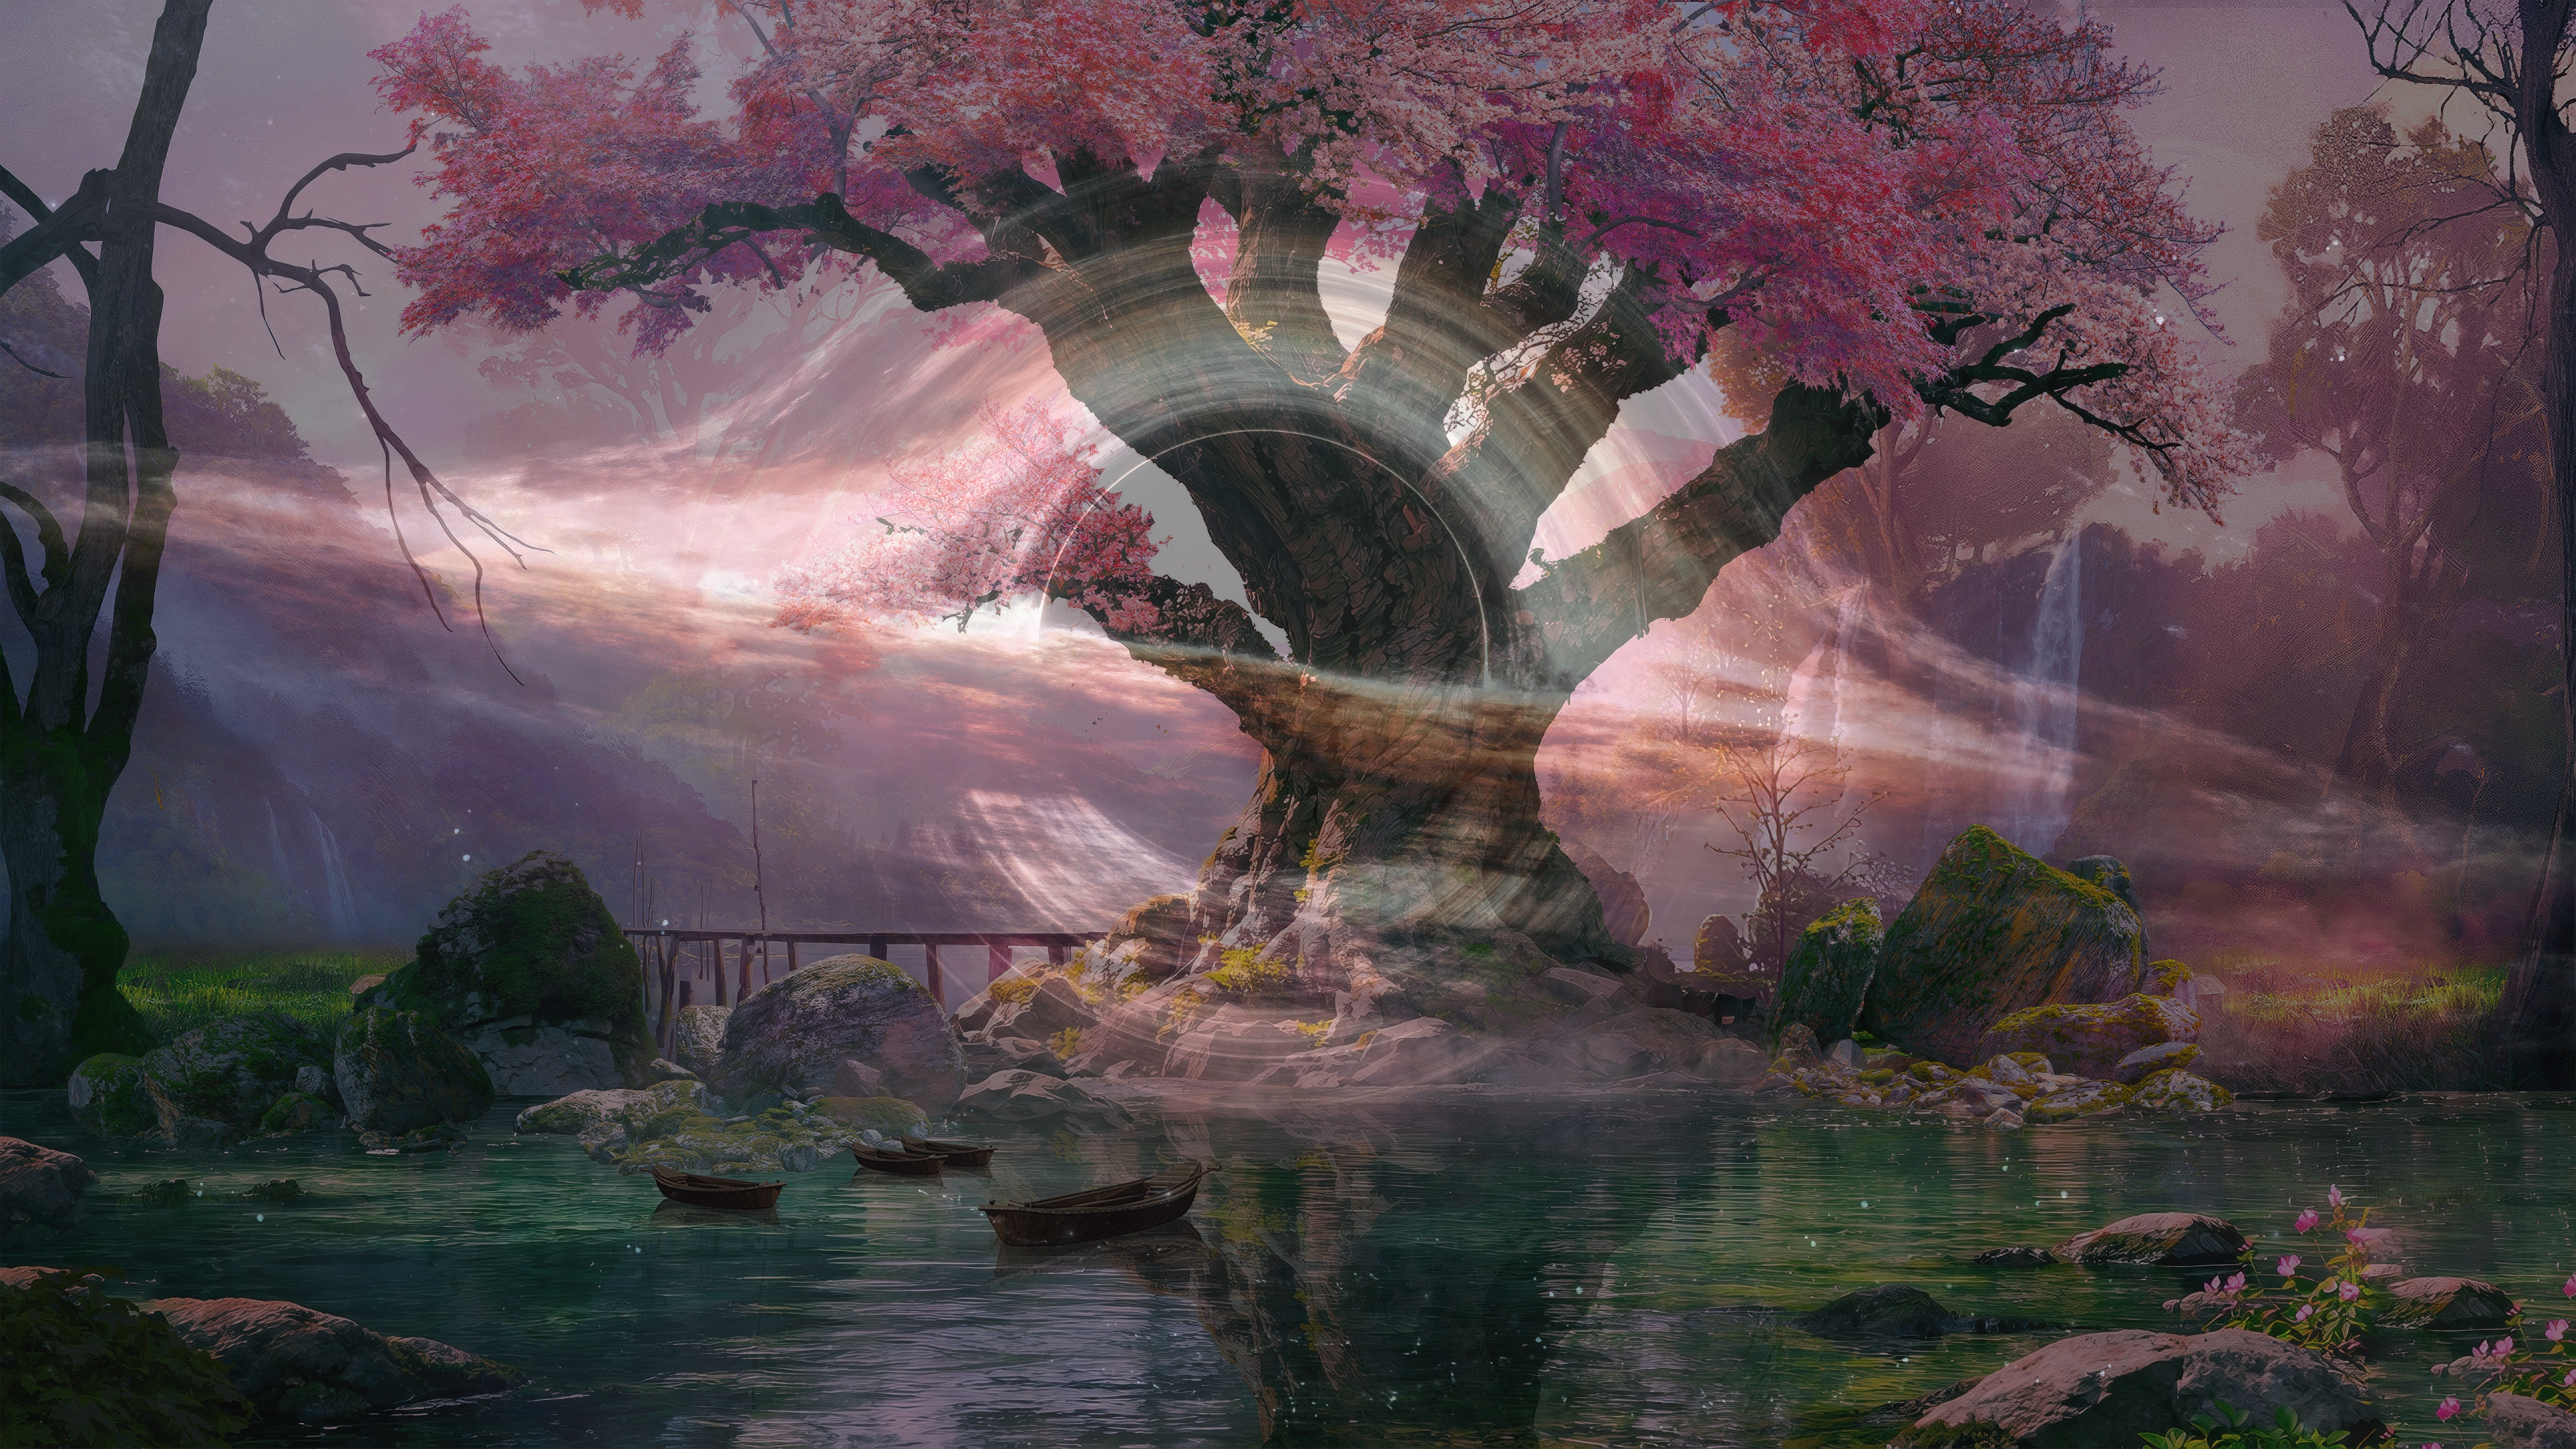
\includegraphics[width=\textwidth]{blend_0.5.png}
\caption{$c = 0.5$}
\end{subfigure}
\hfill
\begin{subfigure}{0.32\textwidth}
\centering
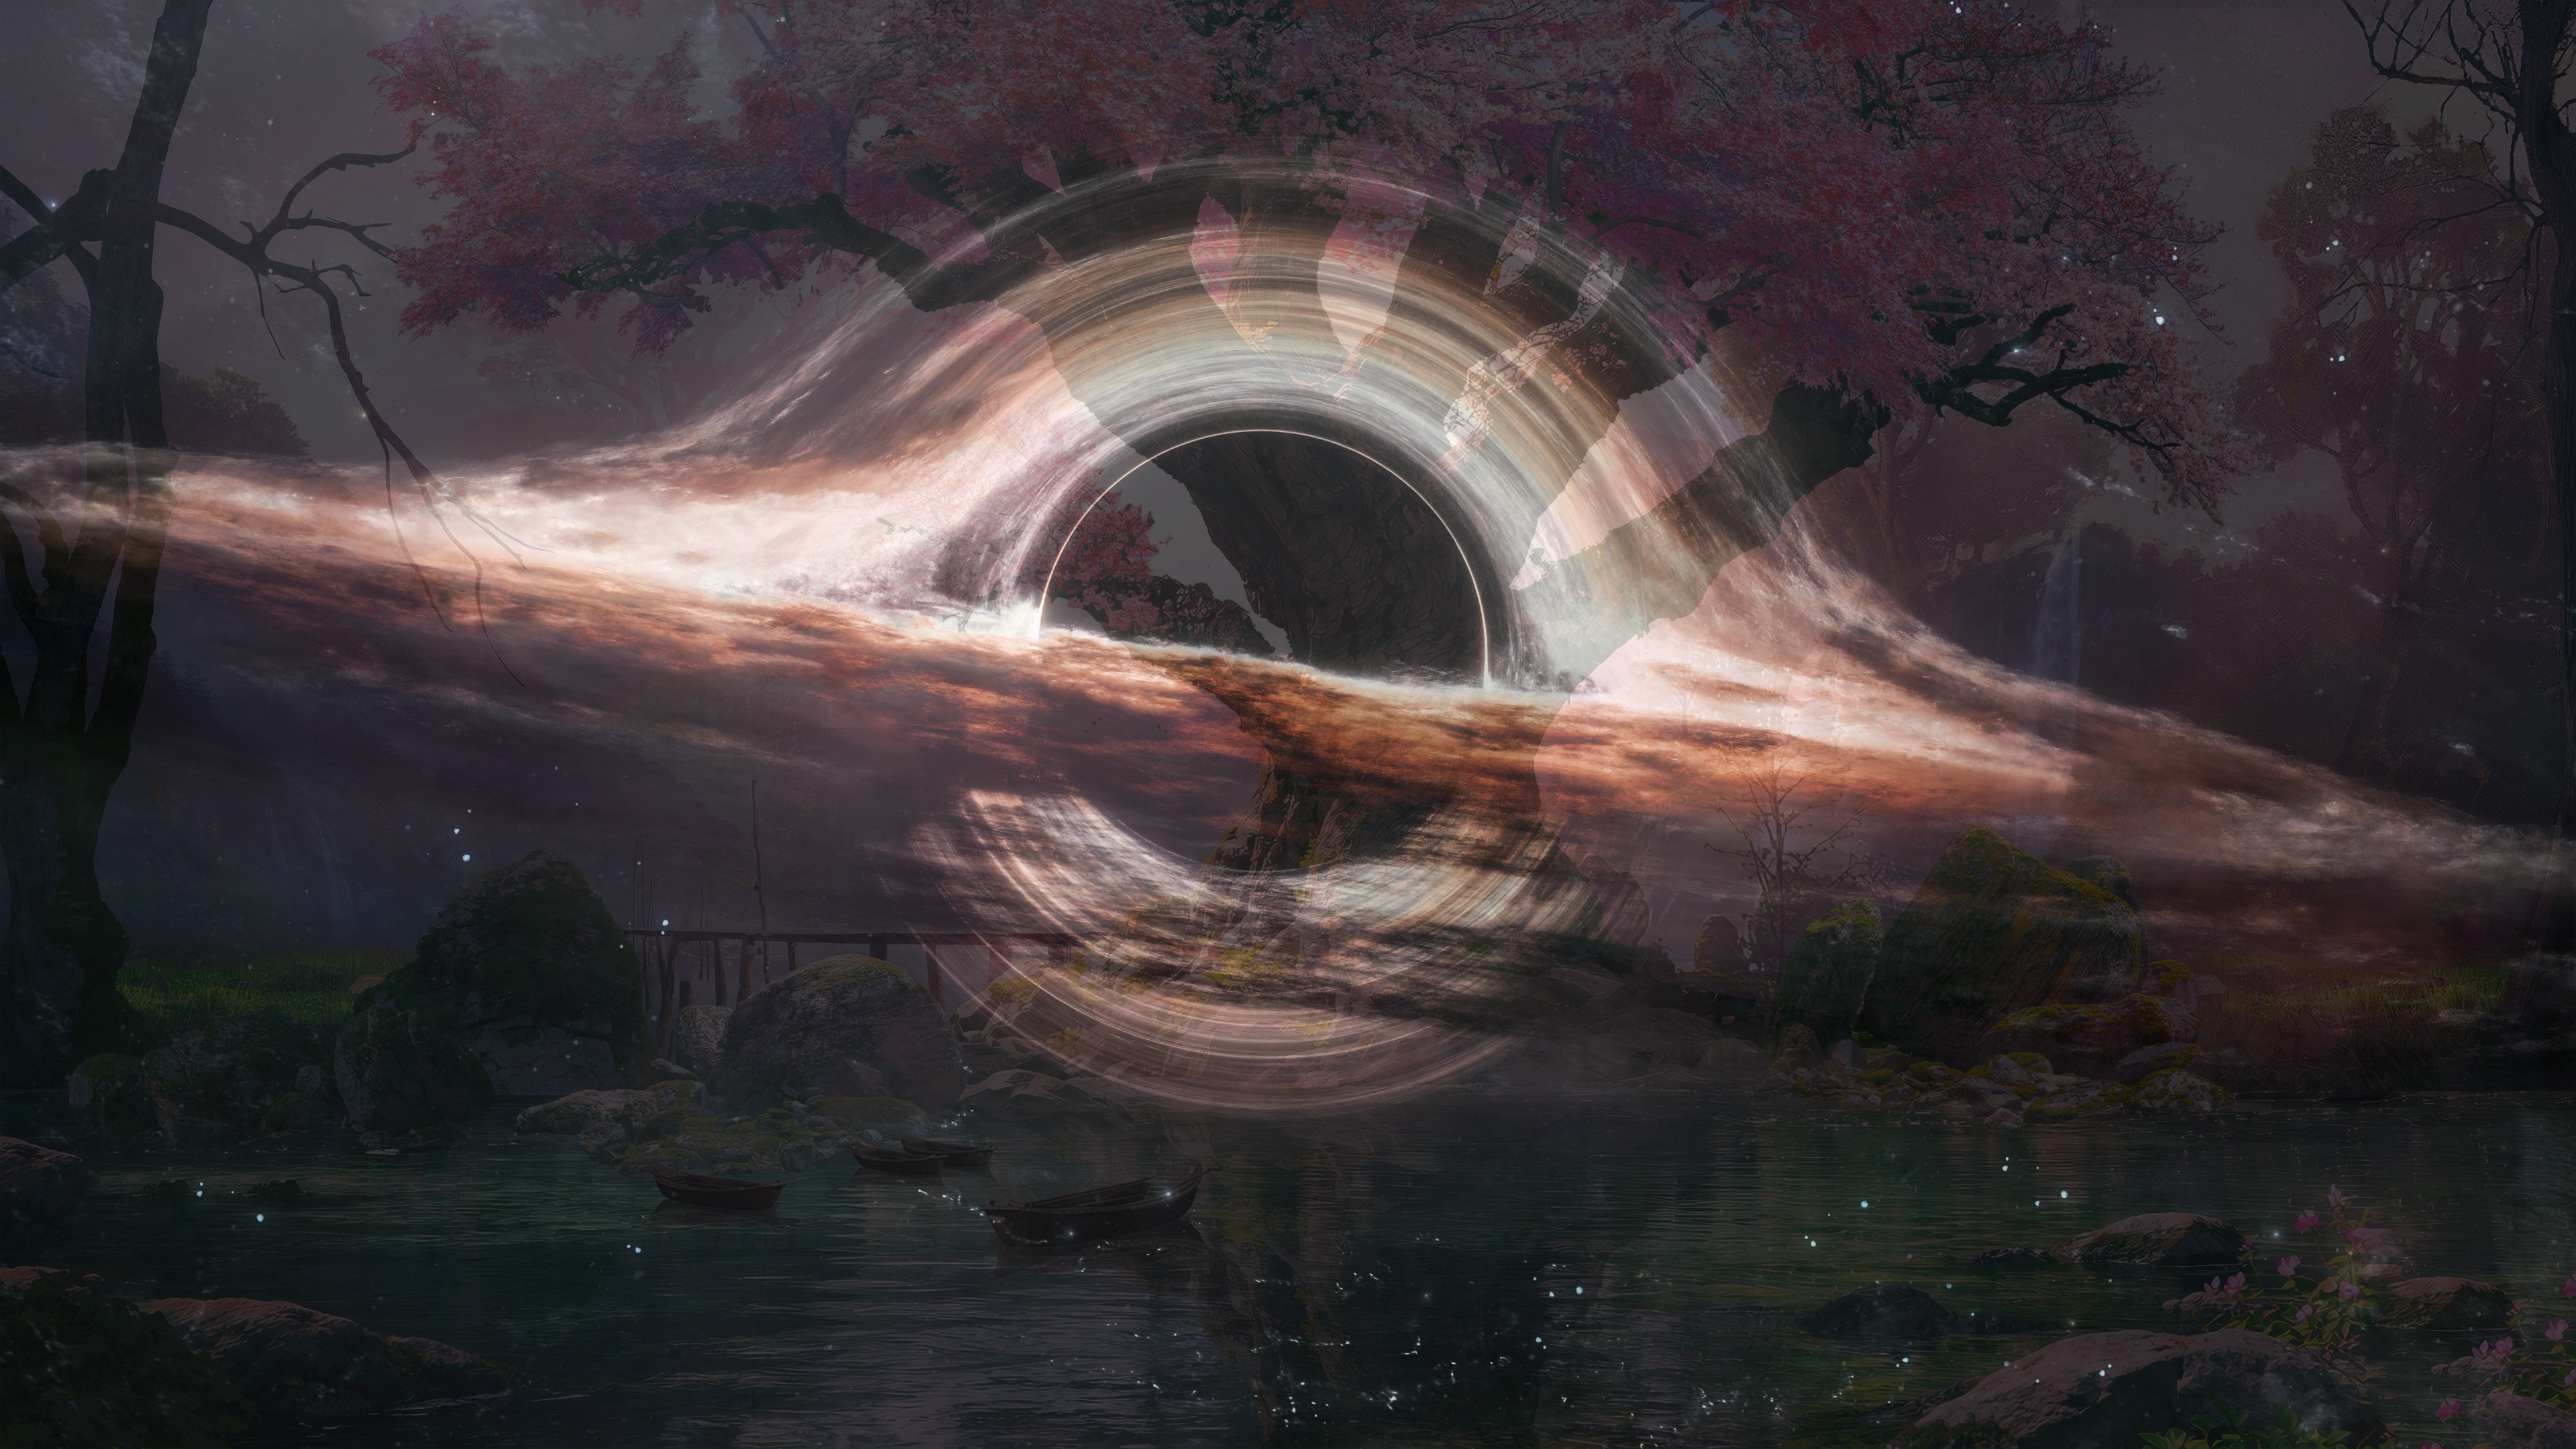
\includegraphics[width=\textwidth]{blend_0.8.png}
\caption{$c = 0.8$}
\end{subfigure}
\caption{Blended images with different blending factors $c$.}
\end{figure}

\section{Block size}

\begin{figure}[H]
\centering
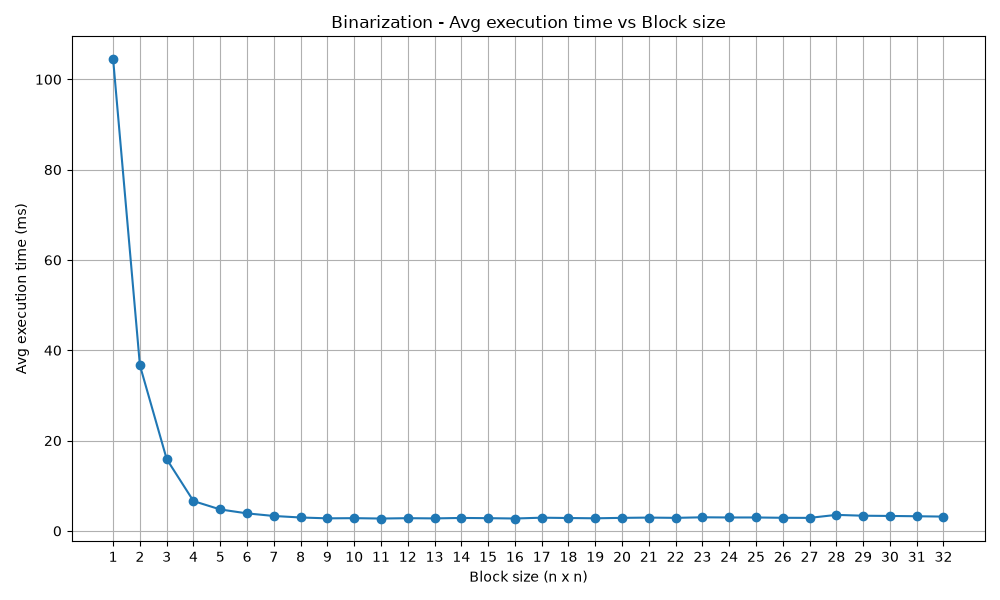
\includegraphics[width=0.7\textwidth]{labwork6a.png}
\caption{Execution times of the image binarization function with different block sizes.}
\end{figure}

\begin{figure}[H]
\centering
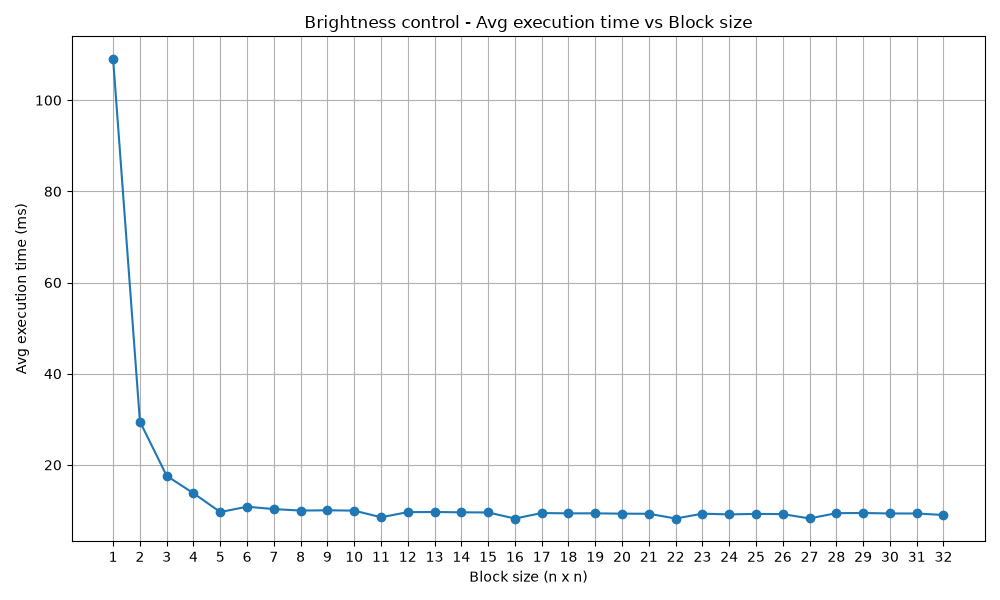
\includegraphics[width=0.7\textwidth]{labwork6b.png}
\caption{Execution times of the image brightness control function with different block sizes.}
\end{figure}

\begin{figure}[H]
\centering
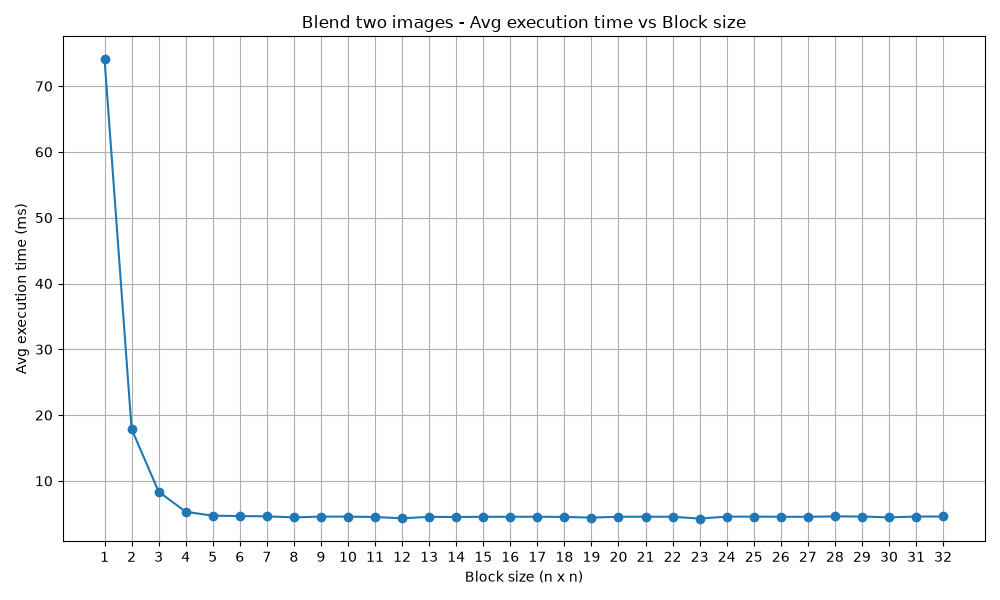
\includegraphics[width=0.7\textwidth]{labwork6c.png}
\caption{Execution times of the image blending function with different block sizes.}
\end{figure}

We can see that like the previous labwork, very small block size are very slow but once we get to like 5x5/6x6 block size, the execution time is low and stays the same until 32x32 block size.

\end{document}